\chapter{Revisão da Literatura}
\label{cap:fundamentacao-teorica}

O estudo das Ondas de Calor Marinhas tem avançado significativamente na última década,
especialmente após a padronização metodológica proposta por \citeonline{Hobday2016}, que estabeleceu
critérios robustos para a detecç~çao e caracterização desses eventos a partir de séries temporais de Temperatura da Superfície do Mar (TSM).
A partir dessa abordagem, diversos estudos têm aplicado a metodologia de Hobday et al. para identificar e analisar as ondas de calor marinhas em diferentes regiões do mundo, 
contribuindo para uma compreensão mais abrangente desses fenômenos e seus impactos nos ecossistemas marinhos. 

No contexto do Atlântico Sul, Regina Rodrigues e Aline S. Taschetto (2020) demonstraram um aumento significativo na frequência, duração e intensidade das MHWs, associando
essas mudanças a fatores como o aquecimento global e a variabilidade climática. O estudo de Hobday et al. (2016) também destacou a importância de monitorar as MHWs para entender seus efeitos nos ecossistemas marinhos e na pesca, especialmente em regiões costeiras vulneráveis.
Esses resultados reforçam a importância de compreender não apenas os efeitos locais dessas anomalias, mas também sua possíveis conexões com o sistema climático continental.

A investigação de telecomunicações climáticas, isto é, a relação entre anomalias em regiões oceânicas e respostas atmosféricas remotas, tem sido tradicionalmente conduzida com base em métodos estatísticos clássicos e dinâmicos,
como discutido por John Marshall e R. Alan Plumb (2016). Esses métodos têm sido eficazes para identificar padrões de teleconexão e compreender os mecanismos subjacentes, mas também apresentam limitações, como a dificuldade de capturar relações não lineares complexas e a dependência de pressupostos estatísticos específicos.
No entanto, abordagens mais recentes têm explorado estruturas complexas e não lineares. Nesse contexto, Niklas Boerrs et al. (2019) utilizaram redes complexas para identificar padrões globais de teleconexões associadas a extremos de precipitação, evidenciando a existência de interações de longo alcance no sistema climático.

Paralelamente, o uso de técnicas de aprendizado de máquina (Machine Learning - ML) tem se consolidado como uma abordageme promisisora para modelagem climática, especialmente na captura de relações não lineares e na previsão de eventos extremos. Estudos como o de X. Zhang et al. (2020) demonstraram a eficácia de modelos de ML para prever ondas de calor marinhas, superando métodos tradicionais em termos de precisão e capacidade de generalização.
Estudos como o de Silva et al. (2024) aplicaram algoritmos como Random Forest e Support Vector Regression (SVR) para previsão de precipitação no Brasil, obtendo desempenho superior a métodos tradicionais em determinados cenários.
De modo semelhante, Oliveira et al. (2025) empregaram modelos como XGBoost e abordagens estatísticas multivariadas para previsão mensal de precipitação na Amazônia, destacando o potencial dessas técniccas em contextos regionais.

Além disso, modelos baseados em redes neurais recorrentes, como Long Short-Term Memory (LSTM) e Recurrent Neural Networks (RNN), têm sido amplamente utilizados na modelagem de séries temporais climáticas devido à sua capacidade de capturar dependências temporais de longo prazo. Estudo recentes demonstram sua eficácia na previsão de variáveis meteorológicas, incluindo temperatura e precipitação, espepcialmente quando combibnados com dados de reanálise e variáveis oceânicas.

Apesar desses avanços, ainda existem lacunas importanntes na literatura. Em particular, poucos estudos integram explicitamente: (i) detecção física de MHWs com base em métricas padronizadas; (ii) a análise de teleconexões oceano-atmosferea em escala regional; e (iii) o uso de modelos de aprendizado de máquina para previsão de extremos hidroclimáticos no Sul do Brasil. A maioria dos trabalhos foca isoladamente em previsão estatística ou em análises descritivas, sem explorar de 
forma integrada o potencial preditivo das anomalias oceânicas para eventos extremos continentais, especialmente em regiões como o Sul do Brasil, que é particularmente vulnerável a eventos de precipitação extrema e suas consequências socioeconômicas.

Dessa forma, o presente estudo se diferencia ao combinar a identificação explícita de MHWs no Atlântico Sul, a extração de métricas físico-oceanográficas relevantes e a aplicação de modelos de aprendizado de máquina para previsão de eventos extremos de precipitação no Sul do Brasil. Essa abordagem integrada visa preencher as lacunas existentes na literatura, proporcionando uma compreensão mais abrangente das conexões entre anomalias oceânicas e eventos extremos continentais, 
além de oferecer insights valiosos para a previsão e mitigação dos impactos desses eventos na região.


\section{Ondas de Calor Marinhas (MHWs): avanços recentes}\label{sec:ondas-de-calor-marinhas}

	As ondas de calor marinhas (MHWs) são eventos extremos de temperatura da superfície do mar (TSM) que podem ter impactos significativos nos ecossistemas marinhos e nas comunidades costeiras. De acordo com a definição padronizada por \citeonline{Hobday2016}, uma MHW é um período prolongado de TSM anormalmente alta, que excede um determinado limiar por um número mínimo de dias consecutivos. A detecção e análise das MHWs são essenciais para compreender seus efeitos e desenvolver estratégias de mitigação.

	As Ondas de Calor Marinhas (Marine Heatwaves - MHWs) passaram a ser amplamente investigadas a partir da padronização metodológica proposta por Hobday et al. (2016), que estabeleceu critérios robustos para a detecção e caracterização desses eventos a partir de séries temporais de Temperatura da Superfície do Mar (TSM). Essa abordagem tem sido fundamental para identificar e analisar as MHWs em diferentes regiões do mundo, contribuindo para uma compreensão mais abrangente desses fenômenos e seus impactos nos ecossistemas marinhos.
	Essa caracterização padronizada tem permitido a extração de métricas fundamentais, como duração, intensidade, frequência e extensão espacial.

	A partir desse marco metodológico, a literatura passou a explorar os impactos das MHWs em diferentes escalas, evidenciando sua influência em processos físicos oceânicos, alterações nos fluxos de calor e impactos em ecossistemas marirnhos.
	Além disso, estudos recentes têm destacado o aumento na ocorrência desses eventos, associando-os às mudanças climáticas e ao aquecimeto dos oceanos.


\section{MHWs no Atlântico Sul e variabilidade climática}\label{sec:mhw-atlantico-sul}

	No contexto do Atlântico Sul, estudos como o de Regina Rodrigues e Aline S. Taschetto (2020) demonstraram um aumento significativo na frequência, duração e intensidade das MHWs, associando essas mudanças a fatores como o aquecimento global e a variabilidade climática. O estudo de Hobday et al. (2016) também destacou a importância de monitorar as MHWs para entender seus efeitos nos ecossistemas marinhos e na pesca, especialmente em regiões costeiras vulneráveis.
	
	Esses resultados são particularmente relevantes para a América do Sul, uma vez que o Atlântico Sul desempenha papel fundamental na modulação do clima regional. Alterações na TSM influenciam o balanço de energia oceano-atmosfera, podendo impactar padrões de circulação atmosférica e, consequentemente, regimes de precipitação e temperatura no continente.

	Apesar desses avanços, a maior parte dos estudos concentram-se na caracterização das MHWs, havendo ainda limitações na compreensão de seus impactos remotos, especialmente no que se refere à sua conexão com extremos hidroclimáticos no Sul do Brasil.

	Esses resultados reforçam a importância de compreender não apenas os efeitos locais dessas anomalias, mas também sua possíveis conexões com o sistema climático continental.

\section{Teleconexões oceano-atmosfera e extremos hidroclimáticos}\label{sec:teleconexoes}

	O conceito de teleconexões climáticas refere-se à interação entre anomalias em diferentes regiões do sistema climático frequentemente mediadas por padrões de circulação atmosférica. A base teórica para o entendimento desses processos é amplamente discutida por John Marshall e R. Alan Plumb (2016), que descrevem os mecanismos físicos que goverenam a dinâmica acoplada oceano-atmosfera. que destacam a importância de métodos estatísticos e dinâmicos para identificar padrões de teleconexão e compreender os mecanismos subjacentes. Esses métodos têm sido eficazes para identificar padrões de teleconexão e compreender os mecanismos subjacentes, mas também apresentam limitações, como a dificuldade de capturar relações não lineares complexas e a dependência de pressupostos estatísticos específicos.

	Tradicionalmente, a identificação de teleconexões tem sido realizada por meio de métodos estatísticos lineares, como correlação e regressão. No entanto, esses métodos apresentam limitações na captura de relações não lineares e interações complexas entre variáveis climáticas. 
	
	Nesse contexto, abordagens mais recentes têm explorado estruturas complexas e não lineares. Niklas Boerrs et al. (2019) introduzem uma abordagem baseada em redes complexas para identificar padrões globais de telecomunicações associadas a extremos de precipitação. Os resultados demonstram que eventos extremos podem estar conectados por estruturas de dependência de longa distância, reforçando a necessidade de abordagens mais sofisticadas para análise.
	

\section{Aplicações de aprendizado de máquina na modelagem climática}\label{sec:aplicacoes-ml}

	O uso de técnicas de aprendizado de máquina tem crescido significativamente na área de ciências climáticas, principalmente devido à sua capacidade de modelar relações não lineares e lidar com grandes volumes de dados. Estudos como o de X. Zhang et al. (2020) demonstraram a eficácia de modelos de aprendizado de máquina para prever ondas de calor marinhas, superando métodos tradicionais em termos de precisão e capacidade de generalização. Esses modelos têm se mostrado particularmente úteis na previsão de eventos extremos, onde as relações entre variáveis podem ser altamente complexas e não lineares.

	No contexto brasileiro, Silva et al. (2024) aplicaram algoritmos como Random Forest e Support Vector Regression (SVR) para previsão de precipitação, demonstrando ganhos de desempenho em relação a métodos tradicionais. De forma complementas, Oliveira et al. (2025) utilizaram modelos XGBoost e abordagens estatísticas multivariadas para previsão mensal de precipitação na região amazônica, evidenciando o potencial dessas técnicas em diferentes contextos climáticos.

	Além desses métodos, modelos baseados em redes neurais recorrentes, como Long Short-Term Memory (LSTM) e Recurrent Neural Networks (RNN), têm se destacado na modelagem de séries temporais climáticas. Esses modelos são especialmente eficazes na captura de dependências temporais de longo prazo, sendo amplamente utilizados na previsão de variáveis meteorológicas como temperatura e precipitação.


\section{Detecção e representação computacional de Ondas de Calor Marinhas}\label{sec:deteccao-mhw}

	A identificação de Ondas de Calor Marinhas tornou-se mais consistente a partir da formalização proposta por Alexander J. Hobday et al. (2016), que define esses eventos como consequências temporais de anomalias positivas de Temperatura de Superfície do Mar acima de um limiar percentílico climatológico por, no mínimo, cinco dias consecutivos.

	Do ponto de vista computacional, essa definição transforma a detecção de MHWs em um problema de processamento de séries temporais com limiar dinâmico, no qual é necessário: (i) calcular climatologias móveis; (ii) identificar excedências; (iii) extrair segmentos temporais contínuos; e (iv) derivar atributos, comom duração, intensidade máxima, intensidade acumulada e extensão espacial.

	Essa estrutura permite representar MHWs como objetos temporais parametrizados, viabilizando sua utilização como variáveis explicativas (features) em modelos de aprendizado de máquina.


\section{Variabilidade no Atlântico Sul e geração de features climáticas}\label{sec:variabildade-features} 
	
	No Atlântico Sul, o trabalho de Regina Rodrigues e Aline S. Taschetto (2020) evidencia o aumento na frequência e intensidade das MHWs, associando esses padrões a variabilidades de larga escala.

	Sob a ótica de ciência de dados, esses estudos fornecem uma base importante para a construção de features espapciais e temporais, sendo elas mapas de anomalias de TSM, índices regionais agregados (spatial pooling), métricas de persistência e recorrência e padrões sazonais.

	No entanto, há uma limitação recorrente na literatura, a maioria das análises utiliza agregações estatísticas simples ou regressões lineares, o que reduz a capacidade de capturar interações não lineares e dependências espaço-temporais complexas.

	Isso abre espaço para abordagens baseadas em aprendizado de máquina, capazes de lidar com dados de alta dimensionalidade e estruturas não lineares. 


\section{Modelagem de teleconexões como problema de dependência complexa}\label{sec:modelagem-teleconexoes}

	As teleconexões oceano-atmosfera podem ser interpretadas, do ponto de vista computacional, como um problema de modelagem de dependências entre variáveis espaço-temporais distribuídas. Esses modelos frequentemente apresentam defasagens temporais (lags), relações não lineares e dependências de longa distância (long-range dependencies).
	
	A base física desses processos é discutida por John Marshall e R. Alan Plumb (2016), mas sua modelagem tradicionalmente depende de métodos lineares.

	Avançando nesse sentido, Niklas Boerrs et al. (2019) propõem o uso de redes complexas (complex networks) para representar o sistema climático como um grafo, no qual os nós representam regiões geográficas e as arestas representam dependências estatísticas significativas. Essa abordagem permite identificar padrões globais de conectividade e eventos extremos associados.

	Apesar de inovadora, essa linha apresenta limitações, como a dependência de critérios de significância estatística e a dificuldade de capturar relações não lineares complexas, o que sugere a necessidade de abordagens complementares baseadas em aprendizado de máquina para modelar essas dependências de forma mais robusta.


\section{Aprendizado de máquina aplicado à previsão climática}\label{sec:ml-climatica}

	A aplicação de aprendizado de máquina na previsão de variáveis climáticas tem crescido significativamente, especialmente em problemas de regressão e séries temporais.

	No Brasil, Silva et al. (2024) demonstraram a eficácia de modelos como Random Forest e Support Vector Regression (SVR) na previsão de precipitação, destacando sua capacidade de capturar relações não lineares.
	De modo semelhante, Oliveira et al. (2025) aplicaram XGBoost e modelos estatíticos multivariados na previsão mensal de precipitação na Amazônia.

	Do ponto de vista computacioinal, esses trabalhos evidenciam três aspectos importantes:

	\begin{enumerate}
		[label=(\roman*)]
		\item o uso de modelos baseados em árvores (Random Forest, XGBoost) para lidar com dados de alta dimensionalidade e relações não lineares;
		\item a dependência de feature engineering manual; e
		\item a limitação na modelagem explícita de dependências temporais longas.
	\end{enumerate}


	Nesse contexto, modelos baseados em redes neurais recorrentes, como LSTM e RNN, surgem como alternativas mais adequadas para sérieis temporais climáticas, ao permitirem modelar sequências com memória, capturar padrões de longo prazo e integrar múltiplas variáveis simultaneamente.

	Ainda sim, muitos estudos utilizam essas abordagens de forma isolada, sem incorporar variáveis oceânicas estruturadas, como métricas de MHWs.


\section{Integração entre dados oceânicos e modelos preditivos}\label{sec:integracao}

	Apesar dos avanços nas áreras de MHWs e aprendizado de máquina, há uma lacuna significativa na integração entre dados oceânicos estruturados (e.g. eventos de MHWs), variáveis atmosféricas continentais e modelos preditivos baseados em ML.

	Grande parte dos estudos utilizam apenas dados meteorológicos locais, ignora a estrutura espaço-temporal do oceano ou trata variáveis oceânicas de forma agregada e simplificada.

	Além disso, são poucos os estudos que exploram explicitamente a seleção de features baseada em relevância física, a análise de importância de importância de variáveis (feature importance) e a interpretabilidade dos modelos em contexto climático.

\section{Lacunas na literatura e posicionamento da pesquisa}\label{sec:lacunas}

	Apesar dos avanços observados nas áreas de detecção de MHWs, análise de teleconexões e aplicação de aprendizado de máquina, a literatura ainda apresenta lacunas relevantes.

	Em particular, observa-se escassez de estudos que integrem de forma conjunta:
	
	\begin{enumerate}
		[label=(\roman*)]
		\item a detecção padronizada de MHWs com base em métricas físico-oceanográficas;
		\item a análise de teleconexões oceano-atmosfera com foco regional; e
		\item a aplicação de modelos de aprendizado de máquina para previsão de extremos hidroclimáticos no Sul do Brasil.
	\end{enumerate}

	Grande parte dos trabalhos existentes aborda esses aspectos de modo isolado, limitando a compreensão integrada dos mecanismos que conectam anomalias oceânicas a impactos continentais, especialmente em regiões vulneráveis como o Sul do Brasil, que é frequentemente afetado por eventos de precipitação extrema e suas consequências socioeconômicas.

	Desse modo, a presente pesquisa se insere nesse contexto ao propor uma abordagem integrada que combina a identificação de MHWs no Atlântico Sul, a análise de teleconexões e eo uso de modelos de aprendizado de máquina (Random Forest, LSTM e RNN) para previsão de extremos hidroclimáticos. 
	Essa integração representa uma avanço metodológico e contribui para o desenvolvimento de ferramentas mais robustas de monitoramento e previsão climática regional.



\section{Eventos extremos hidroclimáticos}\label{sec:eventos-extremos}

	Eventos hidroclimáticos constituem manifestações de baixa frequência e alta initensidade dos processos climáticos e hidrológicos, sendo responsáveis por impactos significativos sobre ecossistetmas, recursos hídricos, infraestrutura e atividades socioeconômicas.
	Nas últimas décadas, a crescentet ocorrência desses eventos tem despertado interesse científico devido à sua relação com a variabilidade climática natural e com as mudanças climáticas antropogênicas.

	Tradicionalmente, extremos hidroclimáticos são definidos como ocorrências raras em relação à distribuição estatística observada de uma variável climáticia ou hidrológica específica, como precipitação, temperatura, vazão ou umidade do solo.
	No entanto, a literatutra recente destaca que a definição de extremo depende não apenas da magnitude do evento, mas também do contexto espacial, temporal e socioambiental em que ocorre (citação SLATER, 2021).

	Segundo Slater (2021), a intensificação observada de diversos extremos climáticos ao redor do mundo tem evidenciado limitações de abordagens clássicas baseadas na hipótese de estacionaridade, tornando necessária a adoção de métodos capazes de representas mudanças temporais na frequência, intensidade e duração desses fenômenos.
	Nesse contexto, a compreensão dos extremos hidroclimáticos exige a integração de conceitos estatísticos, físicos e computacionais, especialmente em estudos voltados para previsão e monitoramento climático.

\subsection{Conceito de extremo climático}\label{sec:conceito-extremo}

	Do ponto de vista estatístico, um evento extremo pode ser entendido como uma observação das caudas da distribuição de probabilidade de uma variável climática. Em resumo, trata-se de um valor significativamente superior ou inferior ao comportamento normalmente esperado para determinada região e período do ano.

	A identificação desses eventos pode ser realizada por diferentes abordagens. 
	Uma das mais utilizadas consiste na adoção de limiares percentílicos, como os percentis 90, 95 ou 99 para extremos positivos, e os percentis 10, 5 ou 1 para extremos negativos.
	Outra estratégia amplamente empregada baseia-se no cálculo de anomalias padronizadas por meio do z-score, que mede a distância entree uma observação e a média climatológica em unidades de desvio padrão.

	Além dessas abordagens, a Teoria dos Valores Extremos (Extreme Value Theory - EVT) fornece uma estrutura probabilística específica para modelar eventos raros, permitindo estimar probabilidades associadas a ocorrências de grande magnitude e períodos de retorno.
	Métodos baseados em EVT têm sido amplamente utilizados em estudos hidrológicos e climáticos devido à sua capacidade de representar adequadamente o comportamento das caudas das distribuições.

	A escolha do método de identificação depende das características dos dados, dos objetivos da pesquisa e da escala temporal analisada.
	Em aplicações de aprendizado de máquina, a definição adequada dos extremos é particularmente importante, pois influencia a construção das variáveis-alvo utilizadas no treinamento dos modelos.

\subsection{Extremos de precipitação}\label{sec:extremos-precipitacao}

	Os extremos de precipitação correspondem a eventos caracterizados por valores excepcioinalmentet elevados ou reduzidos de chuva em relação à climatologia local.
	Esses eventos estão entre os principais responsáveis por desastres naturais em diversas regiões do mundo, podendo ocasionar enchentes, inundações, movimentos de massa, perdas agrícolas e crises de abastecimento hídrico.

	Eventos de precipitação extrema frequentemente resultam da interação entre processos atmosféricos de diferentes escalas, incluindo sistemas frontais, ciclones extratropicais, bloqueios atmosféricos, transporte de umidade e teleconexões climáticas.
	A intensidade desses fenômenos pode ser amplificada por condições oceânicas favoráveis, especialmente quando anomalias de temperatura da superfície do mar modificam os fluxos de calor e umidade entrer oceano e atmosfera.

	Por outro lado, extremos negativos de precipitação estão associados a períodos prolongados de déficit hídrico, caracterizando secas meteorológicas e hidrológicas.
	Esses eventos podem produzir impactos duradouros sobre reservatórios, geração de energia, agricultura e abastecimento urbano.

	De acordo com Slater (2021), estudos recentes têm evidenciado alterações significativas na frequência e intensidade de eventos extremos de precipitação em diversas regiões do planeta, reforçando a necessidade de abordagens que considerem a possível não estacionaridade dos registros climáticos.

\subsection{Extremos de temperatura}\label{sec:extremos-temperatura}
	
	Os extremos de temperatura compreendem eventos em que os valores observados se afastam significativamente da climatologia de referência, podendo manifestar-se na forma de ondas de calor ou ondas de frio.

	Ondas de calor são caracterizadas por períodos persistentes de temperaturas acima do padrão esperado para determinada região e estação do ano. Esses eventos estão associados a impactos sobre a saúde humana, produtividade agrícola, demanda energética e funcionamento de ecossistemas.
	Nos últimos anos, diversos estudos têm documentado aumento na frequência, intensidade e duração das ondas de calor em escala global.

	Em contraste, ondas de frio correspondem a episódios prolongados de temperaturas excepcionalmente babixas, capazes de causar prejuízos à agricultura, mortalidade de animais e riscos à saúde pública.
	Embora o aquecimento global tenha contribuído para a redução da frequência de alguns tipos de extremos frios, esses eventos continuam ocorrendo e podem apresentar severidade regional.

	A ocorrência de extremos de temperatura está frequentemente relacionada a padrões de circulação atmosférica em grande escala e a anomalias oceânicas persistentes.
	Dessa forma, compreender a relação entre condições oceânicas e extremos de temperatura constitui um aspecto fundamental para o desenvolvimento de sistemas preditivos baseados em aprendizado de máquina.

\section{Citações bibliográficas}\label{sec:citacoes}

    Esta frase mostra como citar um livro sobre descargas atmosféricas \cite{rakov2003lightning}. Também podem ser citados \textit{sites} como \citeonline{elat2015densidade}. Você precisa escrever o código da referência no arquivo "referencia.bib" dentro da pasta "elementos-pos-textuais". Veja esse, onde estão alguns exemplos que já foram testados.        
	
    Referenciando outro livro \cite{LangtangenLogg2017}. Texto texto texto texto texto texto texto texto texto texto texto texto texto texto texto texto texto texto texto. Texto texto texto texto texto texto texto texto texto texto texto texto texto texto texto texto texto texto texto. Texto texto texto texto texto texto texto texto texto texto texto texto texto texto texto texto texto texto texto. Texto texto texto texto texto texto texto texto texto texto texto texto texto texto texto texto texto texto texto.

    Referenciando outro site \cite{secretaria1999}. Texto texto texto texto texto texto texto texto texto texto texto texto texto texto texto texto texto texto texto. Texto texto texto texto texto texto texto texto texto texto texto texto texto texto texto texto texto texto texto. Texto texto texto texto texto texto texto texto texto texto texto texto texto texto texto texto texto texto texto. Texto texto texto texto texto texto texto texto texto texto texto texto texto texto texto texto texto texto texto. Citando uma norma \cite{NBR10520:2002}.
        
    Citação de duas referências que concordam entre si \cite{Almeida2018,Gondim2017}. Texto texto texto texto texto texto texto texto texto texto texto texto texto texto texto texto texto texto texto. Texto texto texto texto texto texto texto texto texto texto texto texto texto texto texto texto texto texto texto. Texto texto texto texto texto texto texto texto texto texto texto texto texto texto texto texto texto texto texto. Texto texto texto texto texto texto texto texto texto texto texto texto texto texto texto texto texto texto texto texto texto texto texto texto texto texto. Citando um manual \cite{manuais1989}. 
        
    Outro tipo de citação é a citação literal ou direta com mais de três linhas. Este tipo de citação deve ser destacada com recuo de $4~cm$ da margem esquerda com letra menor (tamanho 10), sem aspas e com espaçamento simples.  Para exemplificar esse tipo de citação, considere a afirmação de \citeonline{feitosa2016}:
    \begin{citacao}
        A cultura é o processo através do qual o homem cria o algo onde antes imperava o nada. Esse algo é toda complexidade de criações simbólicas, de sentidos e significados que damos às coisas e ao mundo. Um ``algo'' que não se sustenta se não se entender os processos culturais como mecanismos de mediação entre nós e os fenômenos. Assim, mais do que apenas um elemento da comunicação, a mediação é, por excelência, cultural. As diversas modalidades de mediação são apenas sotaques diferenciados dessa mediação cultural. Assim é a mediação informacional.
    \end{citacao}
        
    A afirmação do parágrafo anterior também pode ser reproduzida com a citação na final como mostra o exemplo a seguir: 
    \begin{citacao}
        A cultura é o processo através do qual o homem cria o algo onde antes imperava o nada. Esse algo é toda complexidade de criações simbólicas, de sentidos e significados que damos às coisas e ao mundo. Um “algo” que não se sustenta se não se entender os processos culturais como mecanismos de mediação entre nós e os fenômenos. Assim, mais do que apenas um elemento da comunicação, a mediação é, por excelência, cultural. As diversas modalidades de mediação são apenas sotaques diferenciados dessa mediação cultural. Assim é a mediação informacional. \cite{feitosa2016}.
    \end{citacao}
        
%Mais exemplos e opções de citações podem ser encontradas em:
%        https://en.wikibooks.org/wiki/LaTeX/Bibliography_Management
%        https://github.com/cfgnunes/latex-cefetmg/blob/master/latex-cefetmg/03-elementos-pos-textuais/apendices.tex            

\section{Inserindo figuras}\label{sec:figuras}
    
    A Figura \ref{fig:reitoria} apresenta a fotografia da reitoria da Universidade Federal do Ceará. Observe a estrutura do código para ver como inserir figuras. No título, comece especificando o tipo de figura. Por exemplo, fotografia, desenho, diagrama, fluxograma, gráfico e etc. O espaçamento entre linhas no título é de $1~pt$ (espaçamento simples), apenas a primeira letra da frase é maiúscula. As demais palavras são escritas com letra maiúsculas somente quando são nomes próprios e não há ponto final. 
    
    As margens do título da figura são delimitadas pelo tamanho da figura. Por isso, procure ajustar o tamanho da figura para preencher a largura delimitada pelas margens esquerda e direita da página que possui $16~cm$ de largura. Não esqueça de indicar fonte da figura. O autor deve evitar deixar figuras pequenas menores do que $7~cm$ de largura.
    
    A posição da figura deve ser o mais próximo logo após ter sido chamada no texto (a figura nunca deve aparecer antes de ter sido anunciada no texto). 
    
    %troque h pelo b ou t para mudar a posição da figura.
 	\begin{figure}[h!] 
   	    \captionsetup{width=16cm}%Da mesma largura que a figura
		\Caption{\label{fig:reitoria} Fotografia da reitoria da Universidade Federal do Ceará}
		\UFCfig{}{
			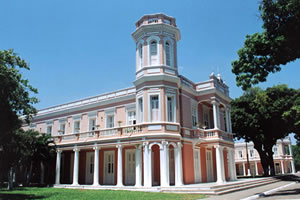
\includegraphics[width=16cm]{figuras/exemplo-1}
		}{
			\Fonte{\citeonline{UFC2012}.}
		}	
	\end{figure}
	
    Texto1 texto texto texto texto texto texto texto texto texto texto texto texto texto texto texto texto texto texto texto texto texto texto texto texto texto texto texto texto texto texto texto texto texto texto texto texto texto texto texto texto texto texto texto texto1.

    Texto2 texto texto texto texto texto texto texto texto texto texto texto texto texto texto texto texto texto texto. Texto texto texto texto texto texto texto texto texto texto texto texto texto texto texto texto texto texto texto2.

    Texto3 texto texto texto texto texto texto texto texto texto texto texto texto texto texto texto texto texto texto. Texto texto texto texto texto texto texto texto texto texto texto texto texto texto texto texto texto texto texto3.

    Texto4 texto texto texto texto texto texto texto texto texto texto texto texto texto texto texto texto texto texto. Texto texto texto texto texto texto texto texto texto texto texto texto texto texto texto texto texto texto texto4.

    A Figura \ref{fig:sondas} Texto texto texto texto texto texto texto texto texto texto texto texto texto texto texto texto texto texto texto. Texto texto texto texto texto texto texto texto texto texto texto texto texto texto texto texto texto texto texto3.

	\begin{figure}[h!]
		\centering
		\captionsetup{width=14cm}%Da mesma largura que a figura
		\Caption{\label{fig:sondas} Gráfico da Atmosfera Superior}	
		\UFCfig{}{
			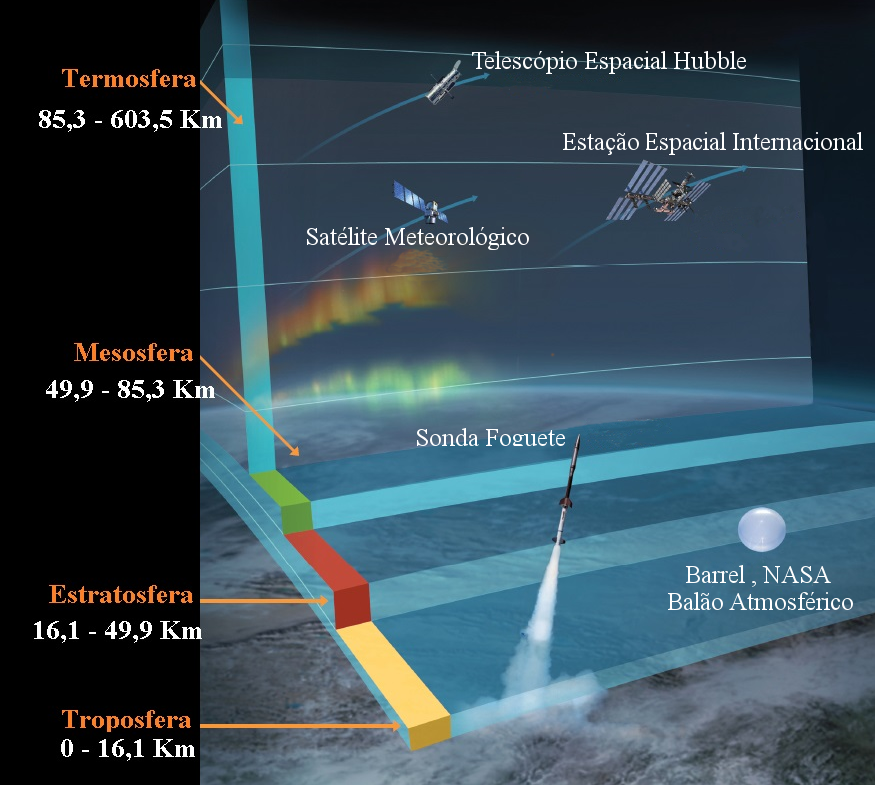
\includegraphics[width=14cm]{figuras/sondas}
		}{
			\Fonte{adaptado da \citeonline{NASA2016}.}}	
	\end{figure}

    Texto5 texto texto texto texto texto texto texto texto texto texto texto texto texto texto texto texto texto texto texto texto texto texto texto texto texto texto texto texto texto texto texto texto texto texto texto texto texto texto texto texto texto texto texto texto5.

    Texto6 texto texto texto texto texto texto texto texto texto texto texto texto texto texto texto texto texto texto texto texto texto texto texto texto texto texto texto texto texto texto texto texto texto texto texto texto texto texto texto texto texto texto texto texto5.

    Texto7 texto texto texto texto texto texto texto texto texto texto texto texto texto texto texto texto texto texto texto texto texto texto texto texto texto texto texto texto texto texto texto texto texto texto texto texto texto texto texto texto texto texto texto texto texto texto texto texto texto texto texto texto texto texto texto texto texto texto texto texto texto texto texto6.

    Evite terminar seções, capítulos e etc com figura. Procure escrever mais.

\section{Inserindo tabelas}\label{sec:tabelas}
    
    A Tabela \ref{tab:exemplo-1}... texto texto texto texto texto texto texto texto texto texto texto texto texto texto texto texto texto texto texto. Texto texto texto texto texto texto texto texto texto texto texto texto texto texto texto texto texto texto texto.
	
	\begin{table}[!h]
	\captionsetup{width=7cm}%Deixe da mesma largura que a tabela
	\Caption{\label{tab:exemplo-1} Um Exemplo de tabela alinhada que pode ser longa ou curta}%
	\IBGEtab{}{%
		\begin{tabular}{ccc}
			\toprule
			Nome & Nascimento & Documento \\
			\midrule \midrule
			Maria da Silva & 11/11/1111 & 111.111.111-11 \\
			Maria da Silva & 11/11/1111 & 111.111.111-11 \\
			Maria da Silva & 11/11/1111 & 111.111.111-11 \\
			\bottomrule
		\end{tabular}%
	}{%
	\Fonte{o autor.}%
	\Nota{esta é uma nota, que diz que os dados são baseados na
		regressão linear.}%
	\Nota[Anotações]{uma anotação adicional, seguida de várias outras.}%
    }
    \end{table}

	%\begin{table}[h!]	
	%	\centering
	%	\Caption{\label{tab:exemplo-1} Exemplo de tabela}	
	%	\UFCtab{}{
	%		\begin{tabular}{cll}
	%			\toprule
	%			Ranking & Exon Coverage & Splice Site Support \\
	%			\midrule \midrule
	%			E1 & Complete coverage by a single transcript & Both splice sites\\
	%			E2 & Complete coverage by more than a single transcript & Both splice sites\\
	%			E3 & Partial coverage & Both splice sites\\
	%			E4 & Partial coverage & One splice site\\
	%			E5 & Complete or partial coverage & No splice sites\\
	%			E6 & No coverage & No splice sites\\
	%			\bottomrule
	%		\end{tabular}
	%	}{
	%	\Fonte{elaborado pelo autor.}
	%}
	%\end{table}

\subsection{Exemplo de subseção} \label{sec:ex_sec}
	
    Texto texto texto texto texto texto texto texto texto texto texto texto texto texto texto texto texto texto texto texto texto texto texto texto texto texto texto texto texto texto texto texto texto texto texto texto texto texto texto texto texto texto texto texto texto.

    %acrlong{DATASUS},\acrlong{DNV},\acrlong{DO},\acrlong{ESF},\acrlong{IBGE},\acrlong{MFC},\acrlong{MI},\acrlong{MS},\acrlong{NV},\acrlong{ODM},\acrlong{OI},\acrlong{OMS},\acrlong{ONU},\acrlong{PNI},\acrlong{PSF},\acrlong{RIPSA},\acrlong{RN},\acrlong{SIM},\acrlong{SINASC},\acrlong{SUS},\acrlong{TMI},\acrlong{TMMFC}


    \begin{alineascomponto}
	    \item Integer non lacinia magna. Aenean tempor lorem tellus, non sodales nisl commodo ut
	    \item Proin mattis placerat risus sit amet laoreet. Praesent sapien arcu, maximus ac fringilla efficitur, vulputate faucibus sem. Donec aliquet velit eros, sit amet elementum dolor pharetra eget
	    \item Integer eget mattis libero. Praesent ex velit, pulvinar at massa vel, fermentum dictum mauris. Ut feugiat accumsan augue, et ultrices ipsum euismod vitae
	    \begin{subalineascomponto}
		    \item Integer non lacinia magna. Aenean tempor lorem tellus, non sodales nisl commodo ut
		    \item Proin mattis placerat risus sit amet laoreet.
	    \end{subalineascomponto}
    \end{alineascomponto}

\subsection{Uso de siglas} \label{sec:siglas}

    Para utilizar siglas, primeiro defina a sigla no arquivo "lista-de-abreviaturas-e-siglas"~ dentro da pasta "1-pre-textuais" com o comando 
    \begin{verbatim}
        \newacronym{ABNT}{ABNT}{Associação Brasileira de Normas Técnicas}
    \end{verbatim}
    Depois chame a sigla com o comando:
    \begin{verbatim}
        \gls{ABNT}
    \end{verbatim}
    Fica assim: \gls{ABNT}. A primeira vez que o comando é usado para uma determinada sigla, aparece o significado por extenso da sigla com a sua abreviação em seguida. A partir da segunda vez que o comando para uma determinada sigla é usado, aparace apenas a sigla. Por exemplo: \gls{ABNT}.  
    
    Veja o código fonte de outros exemplos: Teste de siglas \gls{TEST}, outros exemplos de siglas: \gls{DA}, \gls{MCEG}. 
    Repare que sempre as siglas estão sendo definidas primeiramente no arquivo ``lista-de-abreviaturas-e-siglas''.